
\documentclass[main.tex]{subfiles}
\begin{document}

\chapter{Derivation of the Flow Coefficients}
\label{outflows:sec:coefficients-derivation}

\begin{figure}
\centering
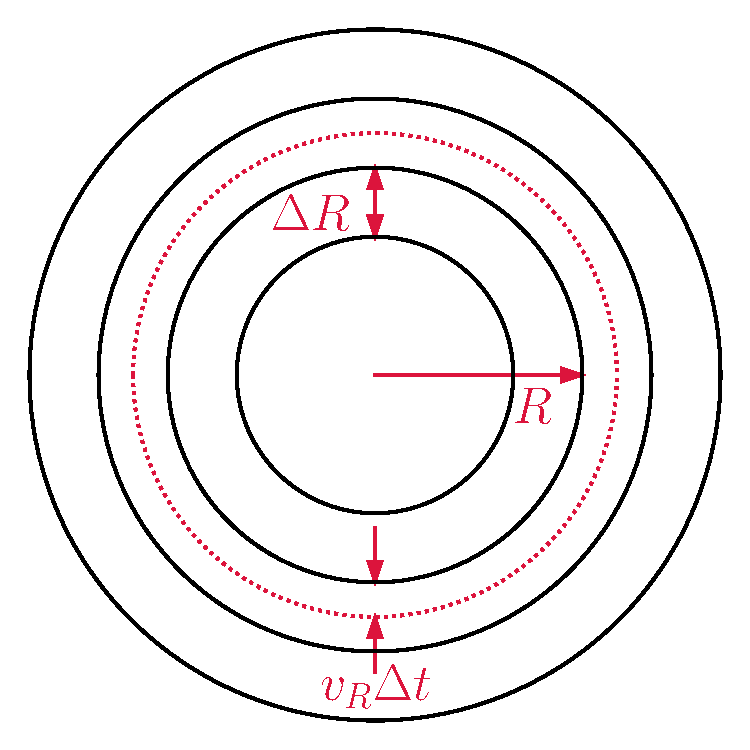
\includegraphics[scale = 0.5]{chapter7/schematic.pdf}
\caption{
A schematic of our derivation of the flow coefficients~$\mu_\flow$
and~$\gamma_\flow$.}
\label{outflows:fig:coefficients-schematic}
\end{figure}

In this Appendix, we present a detailed derivation of the radial gas flow
coefficients~$\gamma_\flow$ and~$\mu_\flow$ given by equations
\refp{outflows:eq:gamma-flow-general} and~\refp{outflows:eq:mu-flow-general}
in~\S~\ref{outflows:sec:gce:onezone}.
We begin by considering a narrow ring embedded in the Milky Way disk spanning
the radial range [$R$, $R + \Delta R$) where the evolution is discretized into
differential timesteps of size~$\Delta t$.
Fig.~\ref{outflows:fig:coefficients-schematic} shows a schematic of this
spatial configuration.
We first derive an expression for the flow rates under this approximation and
subsequently demonstrate that our expressions for~$\gamma_\flow$
and~$\mu_\flow$ arise in the limit that~$\Delta R$,~$\Delta t \rightarrow 0$.
For notational convenience, we define an inward gas velocity to have positive
sign (i.e.,~$v_g > 0$) and simply apply a~$v_g \rightarrow -v_g$ transformation
at the end so that~$v_g > 0$ corresponds to an outward flow according to
convention.
We focus on deriving~$\mu_\flow$ as the form of~$\gamma_\flow$ follows
similarly, but without consideration of the metal mass fraction~$Z_x$.
\par
In the limit of a single, uniform inward flow velocity~$v_g$, all of the ISM
material in the range~$R \rightarrow R + v_g \Delta t$ will be lost to the
next ring inward over the course of one timestep.
The mass that migrates inward can be expressed according to the area fraction
$a$ given by
\begin{equation}
a = \frac{
	2 R v_g \Delta t + v_g^2 \Delta t^2
}{
	2 R \Delta R + \Delta R^2
}.
\label{outflows:eq:area-frac-def}
\end{equation}
Simultaneously, material will be gained from the next ring outward, which spans
radii [$R + \Delta R$, $R + 2\Delta R$).
The net flow rate of some element~$x$ can then be expressed as the difference
of these two source and sink terms:
\begin{equation}\begin{split}
\dot{M}_{x,\flow} &= \dot{M}_{x,\flow,\text{in}} -
\dot{M}_{x,\flow,\text{out}}
\\
&= Z_x(R + \Delta R) M_g(R + \Delta R) \frac{a(R + \Delta R)}{\Delta t} -
Z_x(R) M_g(R) \frac{a(R)}{\Delta t}
\\
&= Z_x(R) M_g(R) \frac{a(R)}{\Delta t}
\left[
\frac{Z_x(R + \Delta R) M_g(R + \Delta R) a(R + \Delta R)}{Z_x(R) M_g(R) a(R)}
- 1\right].
\label{outflows:eq:flowin-minus-flowout}
\end{split}\end{equation}
Regardless of the functional forms of~$Z_x(R)$ and~$M_g(R)$, they can be
expressed as Taylor series, along with~$a$:
\begin{subequations}\begin{align}
Z_x(R + \Delta R) &= Z_x(R) + \sum_{i = 1}^\infty
\frac{\partial^i Z_x}{\partial R^i} \Delta R^i
\\
M_g(R + \Delta R) &= M_g(R) + \sum_{i = 1}^\infty
\frac{\partial^i M_g}{\partial R^i} \Delta R^i
\\
a(R + \Delta R) &= a(R) + \sum_{i = 1}^\infty
\frac{\partial^i a}{\partial R^i} \Delta R^i.
\end{align}\end{subequations}
Although it is straightforward to evaluate~$a(R + \Delta R)$ with
equation~\refp{outflows:eq:area-frac-def}, it is notationally useful for this
derivation to express it as a Taylor expansion.
\par
The flow rate~$\dot{M}_{x,\flow}$ then becomes
\begin{equation}\begin{split}
\dot{M}_{x,\flow} &= Z_x(R) M_g(R)
\frac{2 R v_g + v_g^2 \Delta t}{2 R \Delta R + \Delta R^2}
\Bigg[
\left(1 + \frac{1}{Z_x(R)}
\sum_{i = 1}^\infty \frac{\partial^i Z_x}{\partial R^i} \Delta R^i\right)
\\
&\quad
\left(1 + \frac{1}{M_g(R)}
\sum_{i = 1}^\infty \frac{\partial^i M_g}{\partial R^i} \Delta R^i\right)
\left(1 + \frac{1}{a(R)}
\sum_{i = 1}^\infty \frac{\partial^i a}{\partial R^i} \Delta R^i\right)
- 1\Bigg],
\label{outflows:eq:flowrate-taylor-series}
\end{split}\end{equation}
where we have substituted out~$a(R) / \Delta t$ based on
equation~\refp{outflows:eq:area-frac-def}. 
Taking the limit of this expression as~$\Delta R \rightarrow 0$ requires
L'H\^opital's rule as~$2 R \Delta R + \Delta R^2$ and the expression in square
brackets each approach 0, and we therefore differentiate both of them with
respect to~$\Delta R$.
Briefly using~$\Gamma$ to represent the expression in square brackets for
notational convenience:
\begin{equation}\begin{split}
\frac{\partial \Gamma}{\partial \Delta R} &=
\left(\frac{1}{Z_x} \sum_{i = 1}^\infty i
\frac{\partial^i Z_x}{\partial R^i} \Delta R^{i - 1}\right)
\left(1 + \frac{1}{M_g(R)}
\sum_{i = 1}^\infty \frac{\partial^i M_g}{\partial R^i} \Delta R^i\right)
\\
&\quad
\left(1 + \frac{1}{a(R)}
\sum_{i = 1}^\infty \frac{\partial^i a}{\partial R^i} \Delta R^i\right) +
\\
&\quad
\left(1 + \frac{1}{Z_x(R)}
\sum_{i = 1}^\infty \frac{\partial^i Z_x}{\partial R^i} \Delta R^i\right)
\left(\frac{1}{M_g} \sum_{i = 1}^\infty i
\frac{\partial^i M_g}{\partial R^i} \Delta R^{i - 1}\right)
\\
&\quad
\left(1 + \frac{1}{a(R)}
\sum_{i = 1}^\infty \frac{\partial^i a}{\partial R^i} \Delta R^i\right) +
\\
&\quad
\left(1 + \frac{1}{Z_x(R)}
\sum_{i = 1}^\infty \frac{\partial^i Z_x}{\partial R^i} \Delta R^i\right)
\left(1 + \frac{1}{M_g(R)}
\sum_{i = 1}^\infty \frac{\partial^i M_g}{\partial R^i} \Delta R^i\right)
\\
&\quad
\left(\frac{1}{a} \sum_{i = 1}^\infty i \frac{\partial^i a}{\partial R^i}
\Delta R^{i - 1}\right).
\end{split}\end{equation}
Despite the complicated nature of this expression, the limit as
$\Delta R \rightarrow 0$ results in all terms except those
with~$\Delta R^{i - 1}$ and~$i = 1$ to drop out.
In the denominator, differentiation yields
$2 R \Delta R + \Delta R^2 \rightarrow 2R + \Delta R$, and we arrive at the
following expression for the flow rate:
\begin{equation}
\dot{M}_{x,\flow} = Z_x M_g \frac{2 R v_g + v_g^2 \Delta t}{2R} \left[
\frac{1}{Z_x} \frac{\partial Z_x}{\partial R} +
\frac{1}{M_g} \frac{\partial M_g}{\partial R} +
\lim_{\Delta R \rightarrow 0} \frac{1}{a} \frac{\partial a}{\partial R}
\right].
\end{equation}
\par
Now applying the limit as the timestep size~$\Delta t \rightarrow 0$, it is
straightforward to demonstrate that
\begin{equation}
\lim_{\Delta R, \Delta t \rightarrow 0} \frac{1}{a}
\frac{\partial a}{\partial R} = \frac{1}{v_g} \frac{\partial v_g}{\partial R}.
\end{equation}
This limit must be taken simultaneously since~$a$ depends on both~$\delta R$
and~$\Delta t$.
It is also straightfoward to show that
\begin{equation}
\frac{1}{M_g} \frac{\partial M_g}{\partial R} = \frac{1}{R} +
\frac{1}{\Sigma_g} \frac{\partial \Sigma_g}{\partial R}.
\end{equation}
Combining terms, we arrive at the following expression:
\begin{equation}
\dot{M}_{x,\flow} = -Z_x \dot{M}_\star \tau_\star v_g
\left[
\frac{1}{R} +
\frac{\partial \ln \Sigma_g}{\partial R} +
\frac{\partial \ln v_g}{\partial R} +
\frac{\partial \ln Z_x}{\partial R}
\right],
\end{equation}
where we have additionally substituted in~$M_g = \dot{M}_\star \tau_\star$ to
express the flow rate in terms of the SFR as
in~\S~\ref{outflows:sec:gce:onezone} and applied the transformation
$v_g \rightarrow -v_g$.
\par
As mentioned at the beginning of this Appendix, deriving an expression for the
gas flow rate~$\dot{M}_g$ follows similarly.
The only difference is that no consideration for the metal mass fraction
$Z_x$ is required.
Alternatively, its form can be easily deduced by simply setting~$Z_x = 1$ at
all radii:
\begin{equation}
\dot{M}_{g,\flow} = -\dot{M}_\star \tau_\star v_g \left[
\frac{1}{R} +
\frac{\partial \ln \Sigma_g}{\partial R} +
\frac{\partial \ln v_g}{\partial R}
\right].
\end{equation}
At this point, the proper forms of the flow coefficients~$\gamma_\flow$
and~$\mu_\flow$ given by equations~\refp{outflows:eq:gamma-flow-general}
and~\refp{outflows:eq:mu-flow-general} are now clear.

\end{document}

